\chapter{Note on energy usage}\label{apdx.energy}


\begin{figure}
\begin{center}
\centerline{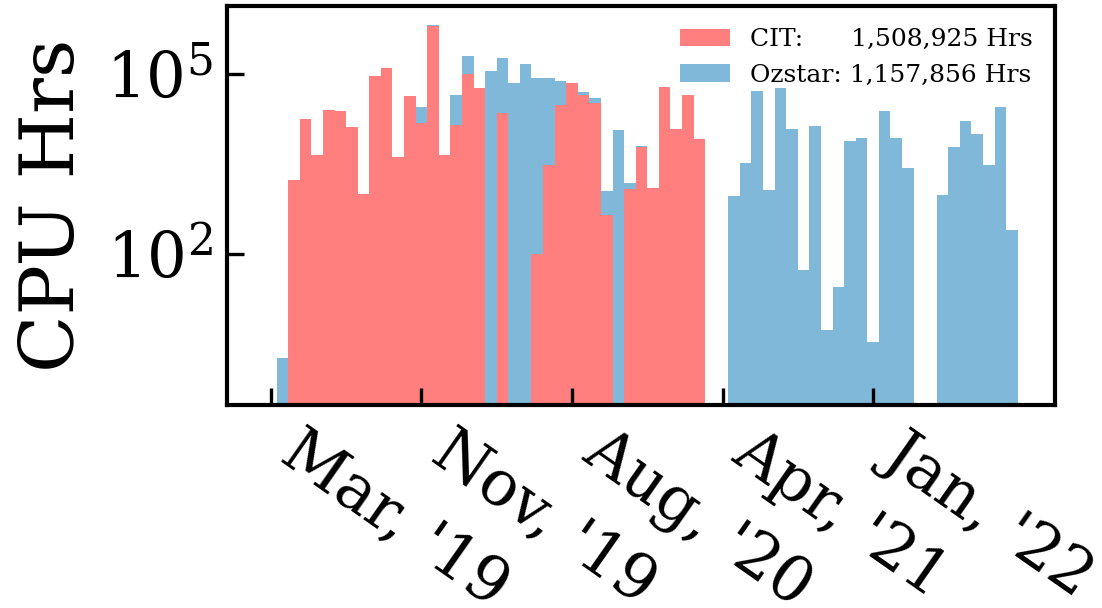
\includegraphics[width=0.75\linewidth]{figures/cpuhrs_timeseries.png}}
  \caption{\textbf{Supercomputer usage:} A stacked bar plot of the supercomputing hours used in this thesis from 2019-22.}\label{fig:computing}
\end{center}
\end{figure}

Supercomputers have enabled scientists to analyse large datasets. However, their power requirements can equate to those of a small city. Scientists must be cognizant of the energy requirements of supercomputers and make efficient use of them.  This will aid in reducing the environmental impact of these powerful machines. To reflect on this, we can paraphrase the famous quote: 
% \myblockquote{With great (supercomputing) power, there must also come --  great responsibility. }{Stan Lee:  Amazing Fantasy \#15, Spider Man,  Vol. 1}

\hspace*{2em}\emph{`With great (supercomputing) power, there must also come --  great responsibility. '}\hspace*{2em}\hfill(Stan Lee:  Amazing Fantasy \#15, Spider Man,  Vol. 1)


During my dissertation, I have used two computing clusters, the California Institute of Technology computing cluster (CIT) and the Swinburne Supercomputing OzSTAR Facility. Figure~\ref{fig:computing} displays the CPU hours I have used from March 2019 to September 2022. All analyses (inclusive of test and failed analyses) performed for this thesis used ${\sim2.6\mathrm{M}}$ core-hours. This includes analyses conducted for the LVK.

Fortunately, as OzSTAR is powered by wind energy from Iberdrola Australia; the electricity for computations produces negligible carbon waste.
However, it is difficult to obtain information about the energy source powering CIT.
Assuming that ${\sim100\ \text{Wh}}$ is required to run and cool each CIT CPU, $\sim1.5\mathrm{M}$ CIT core-hours amount to a carbon footprint of ${\sim50\ \mathrm{t}}$ of ${\text{CO}_2}$ (using the U.S. average electricity source emissions of ${\sim0.4\ \text{kg/kWh}}$~\cite{greenhouse}).
This is roughly equivalent to the annual ${\text{CO}_2}$  output of $\sim30$ Australian households~\cite{}.










\begin{figure}
\begin{center}
\centerline{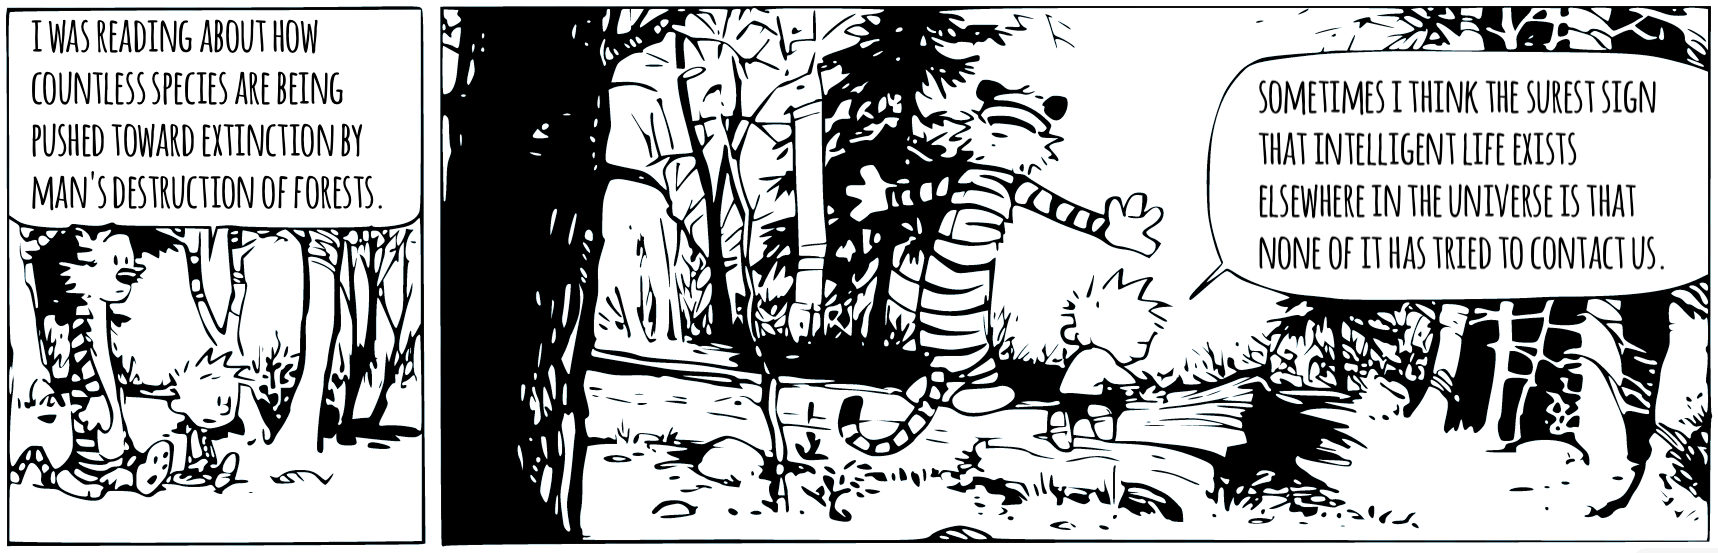
\includegraphics[width=1\linewidth]{figures/calvin_and_hobbes_2.png}}
  \caption*{\tiny CALVIN AND HOBBES \textcopyright\  Watterson. Reprinted with permission of ANDREWS MCMEEL SYNDICATION.}
\end{center}
\end{figure}